\section{Research Goals}

\begin{figure}
	\centering
	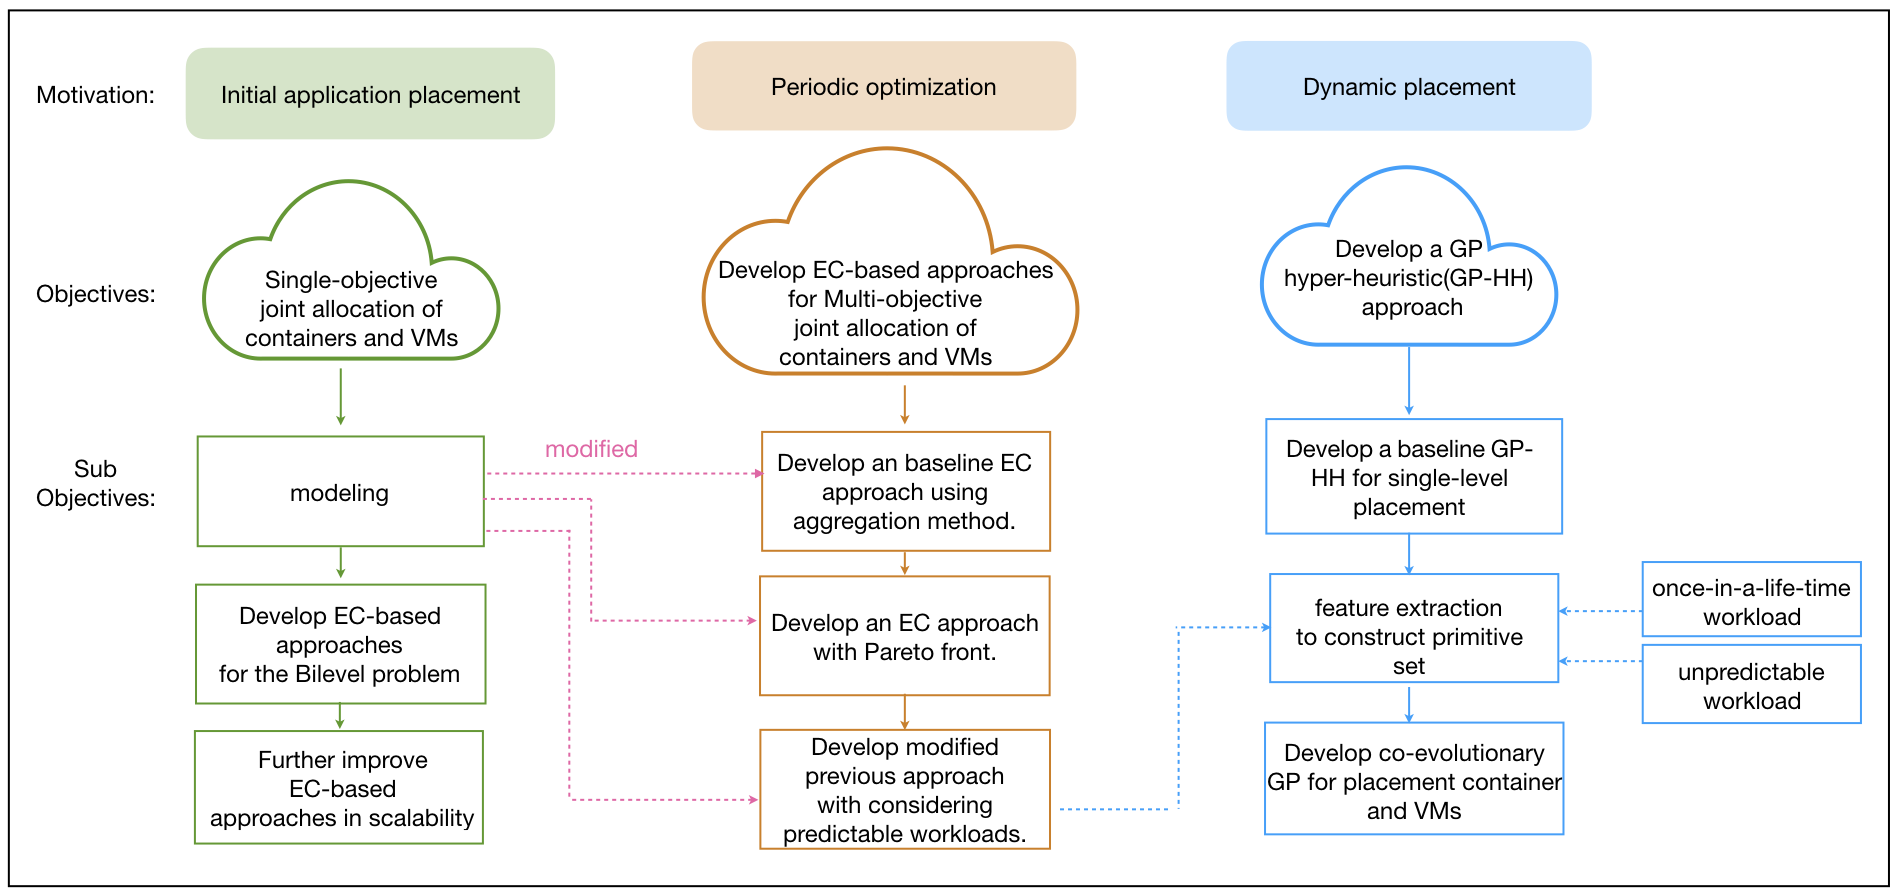
\includegraphics[width=\textwidth]{pics/thesisPlan.png}
	\caption{Relationship between objectives}
	\label{fig:objectives}
\end{figure}
\bx{The overall goal of this research is to optimize energy consumption in container-based clouds using EC-based approaches for three different scenarios:} initial placement of applications, periodic placement of applications, and dynamic placement of applications. The specific research objectives of this work can be itemized as follows.


\subsection{Objective One: Develop EC-based approaches for the single-objective joint placement of containers and VMs for initial placement of applications}
\label{sec:obj1}

\bx{The goal of objective one is to minimize energy consumption in initial placement of applications in container-based clouds.} We set three sub-objectives to achieve this goal. 
For the sake of brevity and without loss of clarity, we will use ``the bilevel model/problem'' to replace ``the joint placement of containers and VMs model/problem'' in the following content. 

\begin{itemize}
	\item Sub-objective 1.1: To develop a new bilevel energy model to represent the relationship between five factors and energy consumption. The five factors involve locations of container, types of VM, locations of VM, overheads of VM, and the balance between memory and CPU. We need to consider the interaction between these factors.


	\bx{The major challenge of designing an energy model for container-based clouds is that the bilevel energy model is more complicated than a single-level energy model in VM-based clouds.}
	\textbf{First}, in VM-based clouds, the only factor is the locations of VMs in PMs. In contrast, in container-based clouds,  the energy model involves four more variables. Specifically, locations of containers decide the utilization of VMs. Types of VMs constrain the placement of containers. Overheads of VMs bring extra workloads to the PMs. The balance of CPU and memory may indirectly impact on the energy consumption. Mishra \cite{Mishra:2011bz} finds better balance leads to a higher probability of allocating more applications. The above mentioned five factors are very likely to affect the energy consumption. \textbf{Second}, two pairs of interaction have not been considered. The first pair is the interaction between containers and types of VMs. The second pair is the interaction between locations of containers and locations of VMs. Therefore, the energy model for container-based clouds is very complicated.


	\bx{In order to establish a bilevel energy model, we propose to follow three steps and gradually add factors to the model. } Because the correlations between the five factors are complicated, we will study their correlation pair by pair. 
	\textbf{First}, we will consider the relationship between overheads, types of VMs, and numbers of VMs because they are closely related. In order to study the overheads of VMs, we will review some research about VM hypervisors and study the impact of VMs. Our hypothesis is that the overheads have a linear relationship with the numbers of VMs and have no correlation with the types of VMs. The outcome of the study of overheads will be a formulation that describes the relationship between overheads, types of VMs, and numbers of VMs.


	\textbf{Second}, we will consider the balance between CPU and memory in both VM and PM levels. No one has yet considered the balance in container-based clouds. We 
	will first consider formulating the balance in both levels. However, this formulation may have a high computation complexity. Hence, we will consider an aggregation of resources from both levels. Our hypothesis is that the aggregation can also achieve high utilization in PMs. The outcome of the study will be a formulation that describes the balance between CPU and memory in two levels.

	\textbf{Third}, we will consider energy consumption with containers, 
	VMs, and PMs. We will review some work on VM-based clouds \cite{Ferdaus:2014ep, Xu:2010vh, Gao:2013gg}. 
	Existing work on server consolidation in VM-based clouds generally represents resource demands as resource utilization. 
	We can use the similar idea to represent containers. The outcome of the study will be a formulation that describes the relationship among containers, VMs, PMs, and energy consumption of clouds.

	
	\bx{This sub-objective is expected, therefore, to formulate a bilevel energy model to represent the relationship between five factors.}



	% The novel contribution of this sub-objective is 


	\item Sub-objective 1.2: To propose a new EC-based bilevel optimization approach to solve the initial placement of applications to achieve better energy efficiency than VM-based approaches.\\
	% \bx{Based on the proposed bilevel model, the goal of this sub-objective is to develop an approach for the bilevel optimization problem using nested Evolutionary algorithms \cite{Sinha:2017et}.}

	\bx{We need to address two challenges.} \textbf{The first challenge} is to design a representation for an EC-based optimization approach. Current VM-based representations only contain one type of variable while container-based representations contain three types of variables: locations of containers, locations of VMs and types of VMs. Furthermore, current VM-based research generally applies binary representation (use 0 and 1 to represent placement). However, in container-based clouds, we cannot apply binary representation because it is not straightforward to represent bilevel of placement. 
	In addition, it is difficult to design a representation that narrows down the search space of solutions.  \textbf{The second challenge} is to design genetic operators and search mechanisms for an EC-based optimization approach. Since a bilevel optimization problem is known as a NP-hard problem \cite{Mathieu:2011dw}, the landscape of search space is ragged because of non-linearity, non-differentiability, non-convexity etc. Therefore, we need to further explore an effective search mechanism that can quickly locate feasible solutions.

	\bx{In order to address the above challenges, we can learn from some existing approaches and design our bilevel approaches.} For the representation, we can review some VM-based research that uses a direct discrete representation \cite{Xu:2010vh} and an indirect continuous probability representation \cite{Xiong:2014jq}. We can learn from their approaches and then design our own. For example, we design a specific representation in the preliminary work (Section \ref{sec:representation}). Furthermore, in order to quickly locate feasible solutions, we can embed a heuristic (see Section \ref{sec:representation}). 
	Based on the representation, we need to first investigate a few EC-based bilevel optimization algorithms such as Genetic Algorithm (GA)-based approaches: Cooperative coevolution algorithm \cite{Legillon:2012dd}, Particle Swarm Optimization (PSO)-based approaches: Nested PSO \cite{Li:2006br} and others \cite{Angelo:2013ee, Zhu:2006in}. Then, we will choose an algorithm and design the genetic operators of the algorithm. For example, for a GA-based algorithm, initialization operators should generate a diverse set of population. Ideally, the population should contain feasible solutions. We will design a mutation operator to allow the population to explore the entire solution space. We will also design a crossover operator to create better solutions based on the good genes of their parents (previous good solutions).
	


	\bx{We will evaluate our approaches in two ways.} \textbf{First}, in order to find the most suitable representation and EC-based algorithm, we will conduct experiments on different approaches and compare their performances in terms of energy efficiency. \textbf{Second}, we will compare the performance of our algorithm with that of existing approaches for VM-based clouds using a same benchmark dataset \cite{Shen:2015hm}. 

	\bx{This sub-objective is expected to propose an EC-based approach for the initial placement of applications.} We expect this approach to achieve better energy efficiency than existing VM-based approaches \cite{Wilcox:2011ea, Xu:2010vh}.

	\item Sub-objective 1.3: To improve the scalability of the proposed EC-based approach a large number of applications.

	\bx{The major challenge of this task is the scalability of bilevel optimization problems and the long computation time of EC-based approaches \cite{Sinha:2017et}.}

	\bx{We can use two methods: bottom-up and top-down to improve the scalability and decrease the computation time.} \textbf{First}, for the bottom-up method, we can reduce the number of variables by combining small containers
	into large combinations of containers. In the first step, we can use clustering approaches such as K-means \cite{Xie:2011fj} and decision tree to categorize containers into major groups and label them as ``CPU intensive'', ``Memory intensive'' etc. An open question is ``what kind of features should we use in clustering''.  In the second step, we will choose containers from these groups to construct combinations. An open question is ``what combination rule should we use''. Greedy-based rules may be useful to quickly construct combinations. In the third step is to decide the size of the constructed combination. Intuitively, large combinations (fewer variables) lead to lower computation complexity. On the other hand, larger combinations may also lead to lower energy efficiency because the combinations of containers are local. Therefore, we need to find an appropriate trade-off between computation complexity and energy efficiency. 

	\textbf{Second}, for the top-down method, we can separate a large problem into several sub-problems so that they can be solved in parallel. Similar to the bottom-up method, a top-down method, such as divide-and-conquer approaches, also has a trade-off in computation complexity and energy efficiency. We will apply the divide-and-conquer \cite{Bentley:1980dz} approach to split a large problem into sub-problems, which can be easily solved individually. However, the aggregation of results from sub-problems may lead to local optima.  Therefore, we will investigate how to split the problem and the size of sub-problems. 

	\bx{We will evaluate our approach by comparing the energy efficiency and execution time with the previously proposed EC-based approach.}

	\bx{This sub-objective is expected to improve the scalability of the previously proposed EC-based approach for up to one thousand applications without decreasing the energy efficiency.}


\end{itemize}
\subsection{Objective Two: Develop an EC-based approach for the multi-objective periodic placement of applications}
\bx{The goal of the second research objective is to develop a multi-objective EC-based approach for periodic placement of applications at container-based clouds with consideration of various types of workload.} The two objectives to be minimized are the energy consumption and the migration cost.
We set three sub-objectives to achieve this goal. 

\begin{itemize}
	\item Sub-objective 2.1: To propose a multi-objective bilevel model for periodic placement with consideration of static workloads.  It has two objectives to be optimized: minimizing the energy consumption and minimizing the migration cost. \\

	\bx{The main challenge is that the cost model in container-based clouds is much complicated than the cost model in VM-based clouds.}
	\textbf{First}, in VM-based clouds, many research only considers the number of migrations \cite{Murtazaev:2014eo} in the cost model. In container-based clouds, because the sizes of containers vary in a wide range (e.g from MBs to GBs), it is inappropriate to simplify the migration cost as the number of migrations. Therefore, we will consider more factors such as network bandwidth to model the migration cost. \textbf{Second}, the container-based cost model not only considers migration of VMs, but also the migration of containers. Therefore, this is a difficult task.

	\bx{In order to solve these challenges,} we will thoroughly study the differences of migration between VMs and containers. For example, a VM contains an OS and all applications' data while a container only includes data of an application. Then, we will explore some VM-based cost models that consider the size of VMs and network bandwidth. We will consider to use a uniform model to represent the  cost of migrating VMs and containers.

	\bx{This sub-objective is expected to formulate the bilevel model to represent both energy consumption and migration cost in container-based clouds.}


	\item Sub-objective 2.2: To propose a multi-objective EC-based bilevel optimization algorithm for periodic placement of applications with a Pareto front approach to achieve better performance than VM-based approaches in both energy efficiency and migration cost.\\

	\bx{We need to solve three challenges.} \textbf{First}, the relationship between the two optimization objectives is very complicated. Since both migration cost and energy consumption can be non-convex, we cannot easily imagine the trade-off between two objectives. \textbf{Second}, we will design genetic operators in an EC algorithm to adapt the bilevel multi-objective optimization. Specifically, genetic operators in both levels collaborate with each other. Hence, it is more difficult to design the collaboration of operators between two levels: containers-VMs and VMs-PMs.  \textbf{Third}, after obtaining a set of non-dominated solutions, we need to further design a fitness function assessment \cite{Moritz:2015hv}. The assessment selects one solution from a large number of non-dominated solutions based on some predefined preferences from cloud providers. The selection of a solution can be a difficult task for a large size of non-dominated set \cite{Zio:2012jz}. 

	\bx{We will follow three steps to address the above challenges.} \textbf{First}, to study the relationship between two objectives, we will first analyze the fitness functions of the objectives. For example, it is likely that in the cost model, the migration cost is monotonically increasing with the number of migrations and size of containers. After analyzing the fitness functions, we can visualize the relationship by using a technique called Trade-off region map \cite{Pinheiro:2015eu}. The trade-off region map can identify local and complex relationships between objectives, gaps in the fitness landscape, and regions of interest. \textbf{Second}, we will first choose an EC-based algorithm based on our previous experience from Objective one. Different from Objective one, we will add trade-off control mechanisms such as non-dominated sorting into the genetic operators. \textbf{Third}, in order to design a fitness function for assessing solutions, we will review some priori and posteriori decision making support methods. On one hand, for priori methods, we assume cloud providers have preferences of energy efficiency and lower migration cost.  On the other hand, for posteriori, we can design a clustering algorithm on the solution set and further narrow down solutions \cite{Zio:2011iq}. 
	 % such as Guided Multi-objective Genetic Algorithm \cite{Jat:2011us} and a clustering approach .

	\bx{We will evaluate our algorithm by comparing with existing VM-based approaches on the same benchmark dataset in terms of the energy consumption and migration cost.}

	\bx{This sub-objective is expected to propose a multi-objective bilevel EC-based approach that can achieve better energy efficiency and migration cost than VM-based approaches.}

	% The major challenge in this sub-objective is to design genetic operators so that the proposed algorithm can steer the search close to the correct Pareto front. The aggregation approach proposed in previous sub-objective has some defects such as it cannot find the non-convex solution. A Pareto front approach is able to find a set of trade-off between objectives, therefore, we decide to explore this direction. Currently only a few research \cite{Yin:2000bt, Deb:2009jh,Deb:2010in} focus on bilevel optimization problem. This will be the first time that bilevel optimization with Pareto front approach is applied on a bilevel bin packing problem.
	% However, most of them are designed for continuous problems. Therefore, new representations and operators need to be considered for discrete problem. 

	% The assumptions for this objective, we will start from one dimensional of resource: CPU utilization. We will consider the static workload in this sub-objective because they are common and easy to start with.  We can utilize the representation and problem models from previous objective. However, we need to propose new genetic operators to adapt the multi-objective problem.

	% like the case in single objective problem, we need to develop new representations, genetic operators.
	\item Sub-objective 2.3: To extend the multi-objective bilevel optimization algorithm to adapt three types of predictable workloads \cite{Fehling:2014tl}: static, linear continuously changing, and periodic. \\
	
	\bx{Several research \cite{Verma:2009wi, Fehling:2014tl} mentions the fluctuation of workloads has a heavy impact on  the periodic placement.} Verma \cite{Verma:2009wi} states that treating workloads as static leads to a performance degradation of applications and low utilization of PMs. Verma considers three types of workloads: static, periodic, and unpredictable while Fehling \cite{Fehling:2014tl} considers three types of predictable workload: static, periodic and linear continuously changing, and two types of unpredictable workload: once-in-a-life-time and irregular. We believe Fehling's classification has a better coverage of existing workloads. Thus, we extend periodic placement on predictable workloads: static, periodic, and linear continuously changing to reach a more stable consolidation (less future migrations). Furthermore, because periodic and linear continuously changing workloads have distinct characteristics, for example, peak vs. no-peak, stable vs. unstable (constant mean value). Hence, we will study periodic and linear continuously changing workloads separately.

	\bx{To consider various types of workload, three challenges exist in this sub-objective.}
	\textbf{First}, it is difficult to reduce the dimensionality of raw workload dataset. Since a typical workload dataset may contain thousands of data points, the dimensionality reduction is critical before applying any similarity measure between workloads. \textbf{Second}, it is not trivial to define the similarity between two kinds of workloads. The current research \cite{Verma:2009wi} only gives a correlation based similarity measurement on two workloads while we will measure the resource demand of an arbitrary number of workloads. \textbf{Third} challenge is to design representations and genetic operators to adapt to three types of workloads.

	\bx{To tackle these challenges,} \textbf{first}, we can apply time-series analysis techniques on workloads such as Independent component analysis (ICA) \cite{Hyvarinen:2004vj}. ICA can extract features from large dimensionality of raw data so that three types of workload can be represented according to their features. \textbf{Then}, we can use a clustering technique with a Pearson correlation as its similarity measurement. \textbf{Third}, we will first try to design a uniform representation for all workloads so that all types of workloads can be treated in the same way. Alternatively we can also define a unique representation for each type of workloads. Accordingly, we will design the genetic operators to suit the representations. 


	\bx{The sub-objective is expected to extend a multi-objective bilevel EC-based approach to three types of workload.}
	
	\end{itemize}




\subsection{Objective Three: Develop a single-objective Cooperative Genetic Programming Hyper-heuristic (GP-HH) approach for automatically generating dispatching rules for dynamic placement of applications.}

\bx{The goal of this objective is to develop a cooperative GP-HH algorithm to generate dispatching rules that can be used to achieve both fast placement and global optimization with five types of workloads: static, periodic, linear continuously changing, once-in-a-life-time, and unpredictable.} We set three sub-objectives to achieve this goal step by step. 

\begin{itemize}

	\item Sub-objective 3.1: To develop a GP-based hyper-heuristic (GP-HH) algorithm for automatically generating dispatching rules for the single-level of placement:  VMs to PMs with static workloads. \\

	\bx{There are three reasons for us to develop a GP-HH algorithm for single-level placement.} \textbf{First}, previous dynamic consolidation methods, including both VM-based and container-based, are mostly based on bin-packing heuristics such as First Fit Descending \cite{:2002vv}. As Mann's research \cite{Mann:2015ua} shown, server consolidation is much harder than a bin-packing problem because of multi-dimensional resources and multiple constraints. Therefore, general bin-packing algorithms do not perform well in multiple constraints. \textbf{Second}, GP has been used in automatically generating dispatching rules in many areas such as dynamic job shop scheduling \cite{Nguyen:2014eu} and bin-packing problems \cite{Burke:2006ei}. Therefore, we will propose a GP-HH approach for solving the dynamic consolidation problem. \textbf{Third}, in order to allocate both containers and VMs, we need to develop two GP-HH approaches for single-level of placement: one addresses containers-VMs and the other addresses VMs-PMs. These two GP-HHs cooperate to generate the dispatching rules for the bilevel optimization problem. Therefore, in the first step, we will design a GP-HH for single-level of placement.

	\bx{Two major challenges,} \textbf{first}, it is difficult to design a hyper-heuristics to generate dispatching rules. We will explore meaningful features of static workloads, VMs, and PMs to construct a primitive set. It is uncertain that which feature can contribute to the dispatching rules.  \textbf{Second}, it is even difficult for the generated dispatching rules to reach a global optimal solution because of the trade-off between training accuracy and over-fitting.

	\bx{To gradually handle above challenges,} \textbf{first}, we start from reviewing the literature about manually designed heuristics and simple bin-packing heuristics. These heuristics contain some features of applications and VMs. For example, First Fit algorithm normally considers the remaining resources of PMs as the criteria of selecting a placement. We will also consider other features such as the status of VMs (e.g resource utilization), features of workloads (e.g resource requirement) that may affect the decision of placement. The above features are represented as resource utilization. We will construct a primitive set with the selected features. 
	\textbf{Second}, we will use the default function set and the basic tree representation for constructing the dispatching rules. 
	\textbf{Third}, to train the GP-HH, we will use the solutions from the first objective as the learning sets. We can use ten folds cross-validation technique to prevent over-fitting. 

	\bx{In order to evaluate the automatically generated heuristics, we will use a widely used simulator called CloudSim \cite{2009LNCS.5931...24B}.} We will compare our heuristics to a highly cited work \cite{Beloglazov:2012ji} from Beloglazov who proposes a Best Fit Decreasing heuristic for the energy consumption problem.

	\bx{The sub-objective is expected to propose a GP-HH algorithm for automatically generating dispatching rules for the single-level placement with static workloads.} The generated dispatching rules are expected to achieve an equal or better performance than manually designed heuristics in terms of energy efficiency. 

	\item Sub-objective 3.2: To conduct feature extraction on the three predictable workloads and two unpredictable workloads to construct a new primitive set. \\
	
	\bx{The major challenge is to discover useful features that can represent various workloads.} The first challenge is to identify features from high dimensionality of datasets. The raw workload dataset may contain a large number of data points. It is difficult to extract meaningful features from the data points. The second challenge is to select useful features from a large number of raw features. It is very time consuming to manually examine raw features. The correlations between these raw features bring additional complexities.

	\bx{To solve these challenges, } \textbf{first}, we will review a number of dimensionality reduction techniques. Some possible techniques are sampling, extrema extraction. \textbf{Second}, we will employ the principle component analysis (PCA) technique on the feature set to reduce the number of features. 

	\bx{Classification of various workloads is one of the way to test the extracted features}. If we can differentiate workloads based on the extracted features with a high accuracy (e.g. 95\%), we can use the features to construct new dispatching rules. 

	\bx{The sub-objective is expected to extract a number of features to represent different types of workloads.} We can apply these features to construct a new primitive set for the dispatching rules to deal with all kinds of workloads.



	\item Sub-objective 3.3: To develop a cooperative GP-HH approach for automatically generating dispatching rules for placing both containers and VMs. \\
	\bx{The major challenge is to develop a cooperating procedure between two GP-HHs on two levels.} 
	As the first step, we will consider using two sub-populations to represent two-levels of placement. Each sub-population would be trained to minimize their objectives. The second step,the sub-population in the containers-VMs level will be used in training the VMs-PMs level of placement. 

	\bx{This sub-objective 3 is expected to propose a cooperative GP-HH approach for automatically generating dispatching rules for dynamic placement of applications in container-based clouds.}

	\end{itemize}
